\documentclass[11pt]{article}
\usepackage[
    letterpaper,
    top=0.65in,
    bottom=0.65in,
    left=0.70in,
    right=0.70in
]{geometry}

\usepackage[T1]{fontenc}
\usepackage[utf8]{inputenc}
\usepackage{amsmath,amssymb}
\usepackage{graphicx}
\usepackage{tabularx}
\usepackage{array}
\usepackage{booktabs}
\usepackage{float}
\usepackage[table]{xcolor}
\usepackage{caption}
\usepackage{titlesec}
\usepackage{hyperref}
\usepackage{csquotes}
\usepackage{microtype}

\graphicspath{{fig/}}

\usepackage[
    backend=biber,
    style=authoryear,
    sorting=none,
    giveninits=true,
    maxbibnames=99,
    dashed=false
]{biblatex}
\addbibresource{references.bib}

\DeclareNameAlias{sortname}{family-given}
\DeclareNameAlias{default}{family-given}
\DeclareFieldFormat[article]{title}{#1}
\DeclareFieldFormat[misc]{title}{#1}
\renewbibmacro{in:}{}
\AtEveryBibitem{\clearfield{doi}\clearfield{urldate}}
\AtBeginBibliography{\small}
\setlength{\bibitemsep}{0.35em}

\definecolor{GWBlue}{HTML}{1E4E79}
\hypersetup{
    colorlinks=true,
    linkcolor=GWBlue,
    citecolor=GWBlue,
    urlcolor=GWBlue
}

\titleformat{\section}
{\Large\bfseries\color{GWBlue}}
{\thesection.}
{0.40em}
{}

\titlespacing*{\section}{0pt}{0.70em}{0.28em}

\captionsetup{
    font=small,
    labelfont=bf,
    textfont=it,
    labelsep=period,
    skip=4pt
}

\setlength{\parindent}{0pt}
\setlength{\parskip}{0.30em}


\begin{document}

\begin{titlepage}
    \centering
    \IfFileExists{fig/gwu_logo.pdf}{
        \includegraphics[width=0.32\textwidth]{gwu_logo.pdf}\par
        \vspace{0.75cm}
    }{}

    {\scshape\Large Data Science Program\par}
    \vspace{0.25cm}
    {\large Department of Data Science\par}
    \vspace{0.35cm}
    {\large DATS 6501 -- Capstone Project -- Fall 2026\par}
    \vspace{0.85cm}

    {\huge\bfseries Post-Training Analysis \& Novelty Detection Using\\
    Neural Network Self-Organizing Maps (NNSOM)\par}
    \vspace{0.75cm}

    {\Large\bfseries SOM 15$\times$15 Report\par}
    \vspace{0.30cm}
    {\Large Topology, Representation Structure \& Validation Analysis\par}

    \vspace{0.95cm}
    {\large Capstone -- Group 5\par}
    \vspace{0.20cm}
    {\large Fyrooz Khan\\ Nazish Atta\par}

    \vfill
    The George Washington University\\
    Washington, DC

    \vspace{0.65cm}
    Supervised by\\
    Dr. Amir Jafari\\
    Associate Professor of Data Science
    \vfill
\end{titlepage}

\section{SOM 15$\times$15 Overview}

This phase applies a 15$\times$15 Self-Organizing Map (SOM) to the
84-dimensional \texttt{fc2} representations extracted from the pretrained
MNIST CNN. The SOM was trained with seed 42 on 49,000 training embeddings and
validated on 10,500 held-out validation embeddings. The objective is to examine
whether topology-preserving organization of the learned representation reveals
class structure, density patterns, and localized validation weaknesses
\cite{kohonen1990som,jafari_nnsom}.

\begin{table}[H]
\centering
\begin{tabular}{ll}
\toprule
\textbf{Item} & \textbf{SOM 15$\times$15 Setup} \\
\midrule
Grid & 15 $\times$ 15 neurons (225 units) \\
Random seed & 42 \\
Training samples & 49,000 \\
Validation samples & 10,500 \\
Input representation & CNN \texttt{fc2} embeddings \\
Feature dimension & 84 \\
Class-map split & Validation \\
Top-variance features & 15, 19, 79, 41, 35, 53 \\
\bottomrule
\end{tabular}
\caption{SOM 15$\times$15 experimental metadata.}
\end{table}

\section{SOM Training and Quantization Error}

Quantization error measures how closely samples are represented by their Best
Matching Units (BMUs). The training trace is therefore useful for checking
optimization behavior before interpreting the final map. It should not be
treated as stand-alone evidence of downstream novelty-detection quality.

\begin{figure}[H]
    \centering
    \includegraphics[width=0.88\textwidth]{som_15x15_seed42_final_qe_curve.pdf}
    \caption{SOM quantization error across training for the 15$\times$15 seed-42 run.}
\end{figure}

\section{Topology and Neighborhood Structure}

The topology view establishes the two-dimensional neuron lattice, while the
U-Matrix summarizes distances between neighboring SOM prototypes. Larger
inter-neuron distances can indicate transitions between regions of the learned
representation, making the U-Matrix a central structural diagnostic
\cite{kohonen1990som,vesanto2000clustering}.

\begin{figure}[H]
    \centering
    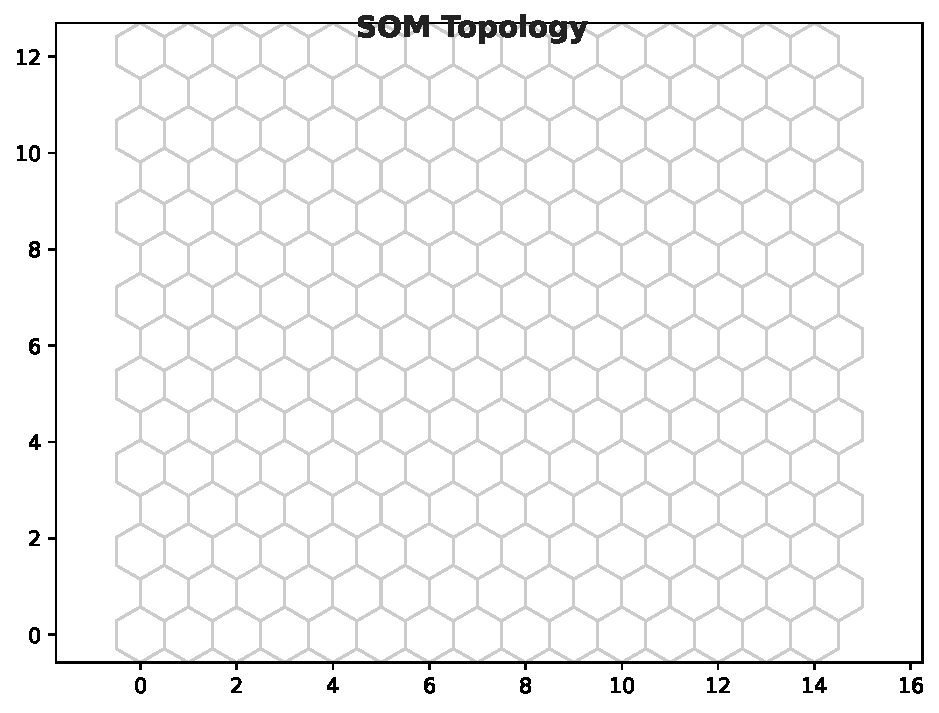
\includegraphics[width=0.47\textwidth]{topology.pdf}
    \hfill
    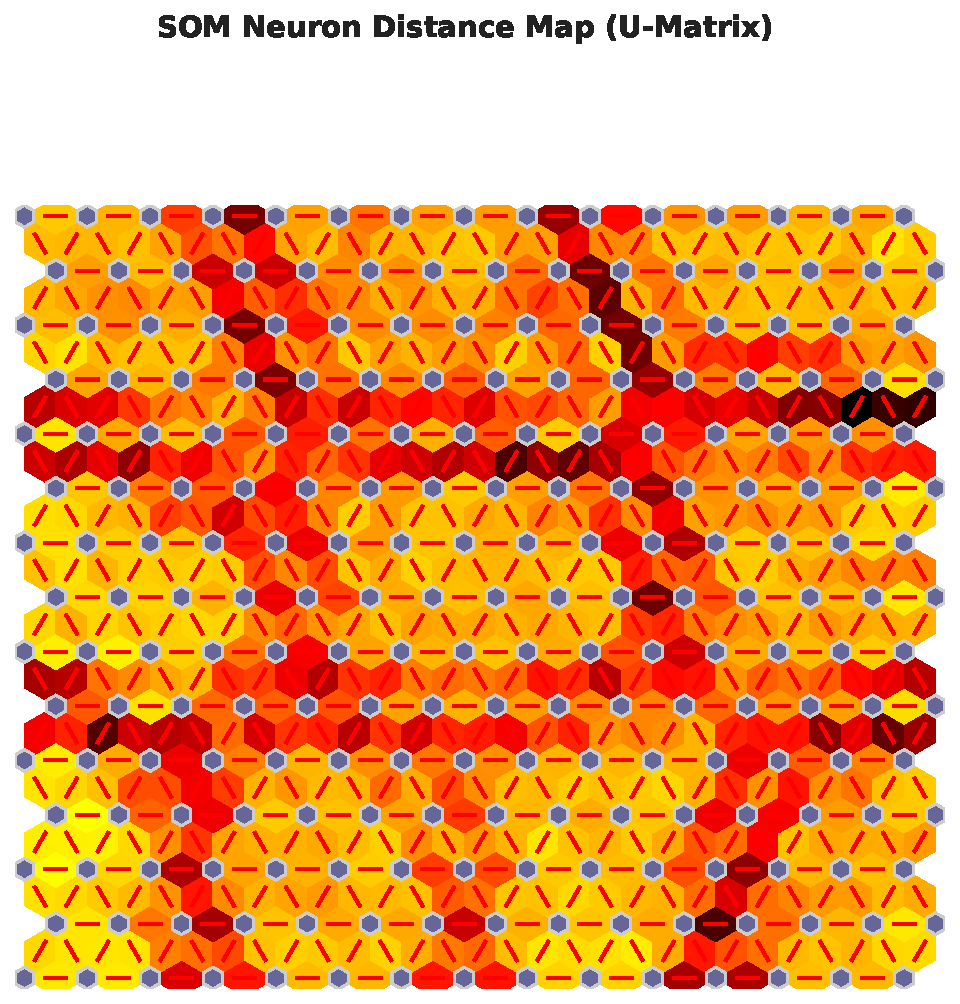
\includegraphics[width=0.47\textwidth]{u_matrix_neuron_distance.pdf}
    \caption{SOM topology (left) and U-Matrix / inter-neuron distance structure (right).}
\end{figure}

\section{Sample Distribution and Hit Maps}

Hit histograms quantify how many samples map to each neuron. Comparing training
and validation occupancy provides a compact view of whether major density
regions are reproduced in held-out data. Differences are descriptive diagnostics
and should not be interpreted as overfitting without quantitative support.

\begin{figure}[H]
    \centering
    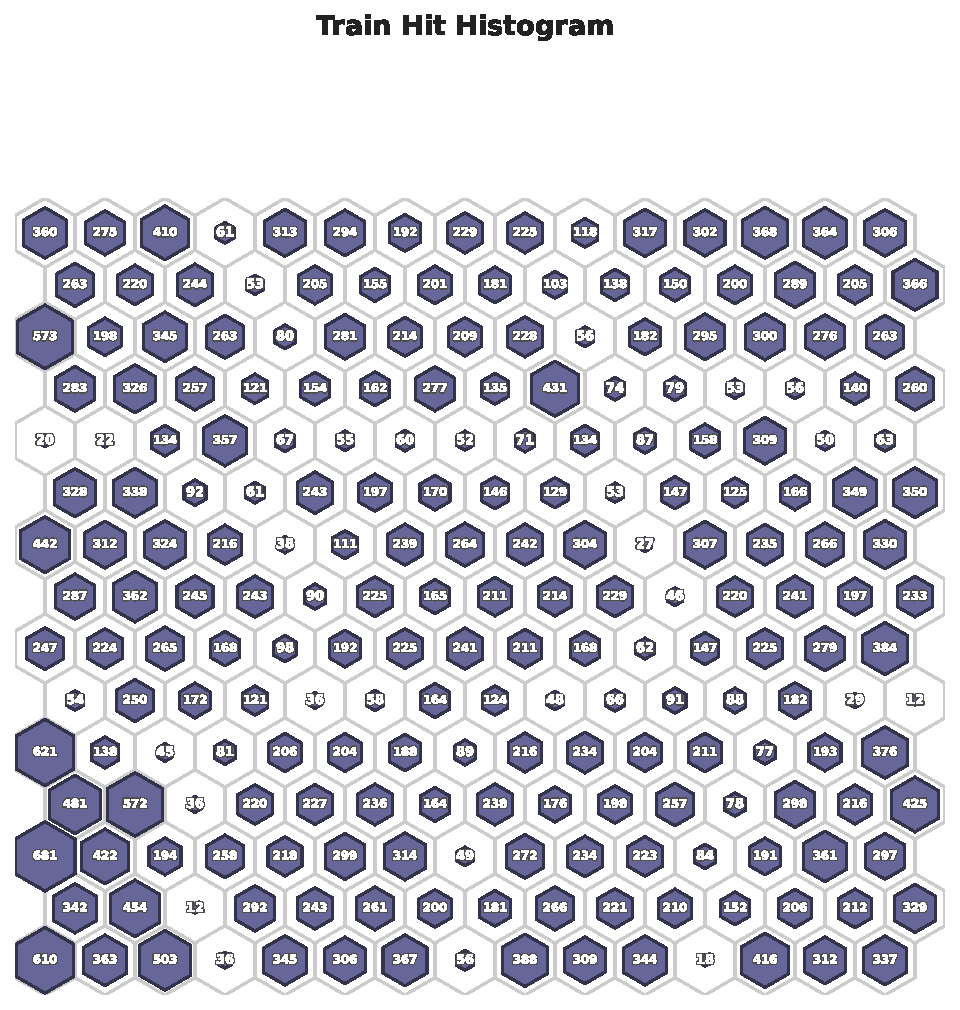
\includegraphics[width=0.47\textwidth]{train_hit_histogram.pdf}
    \hfill
    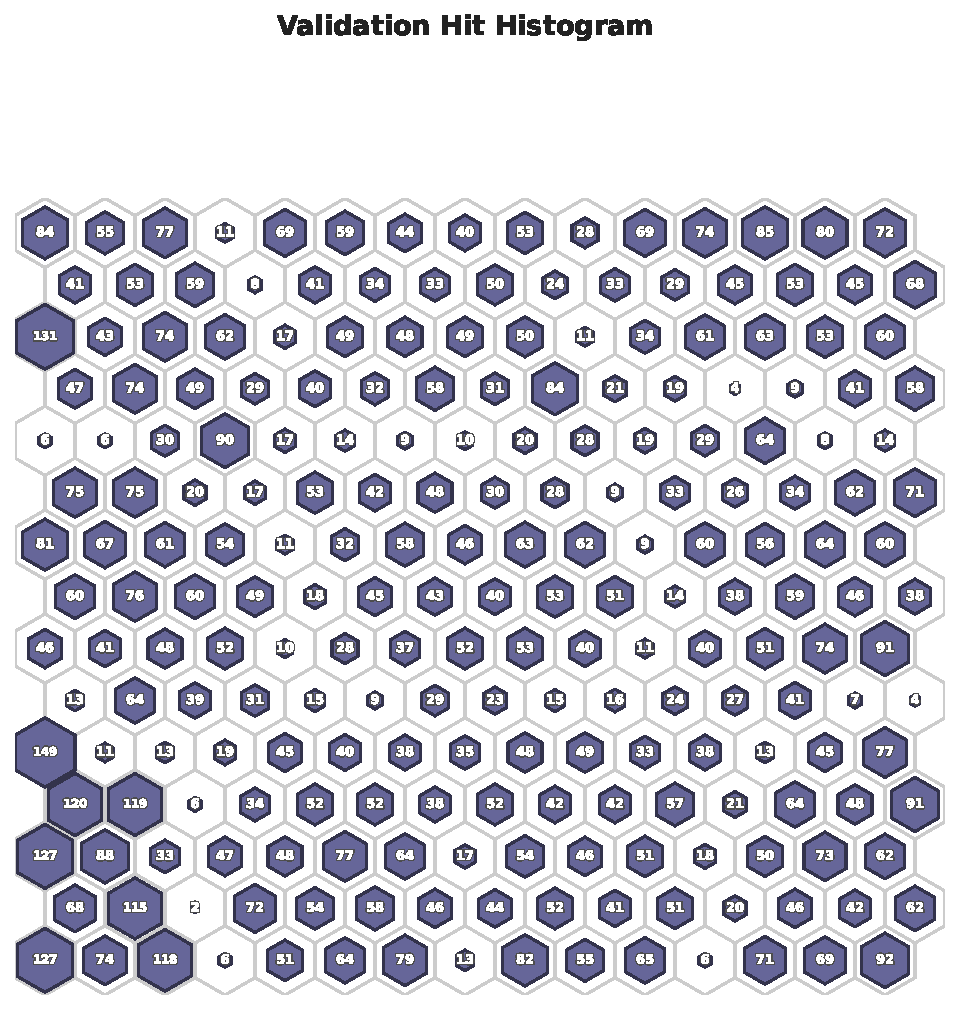
\includegraphics[width=0.47\textwidth]{validation_hit_histogram.pdf}
    \caption{Training and validation SOM hit histograms.}
\end{figure}

\section{Representation Structure}

Component planes show how each input dimension varies across the SOM lattice.
Because the SOM is trained directly on the 84-dimensional \texttt{fc2}
representation, these planes provide a map-level view of how internal CNN
features organize spatially.

\begin{figure}[H]
    \centering
    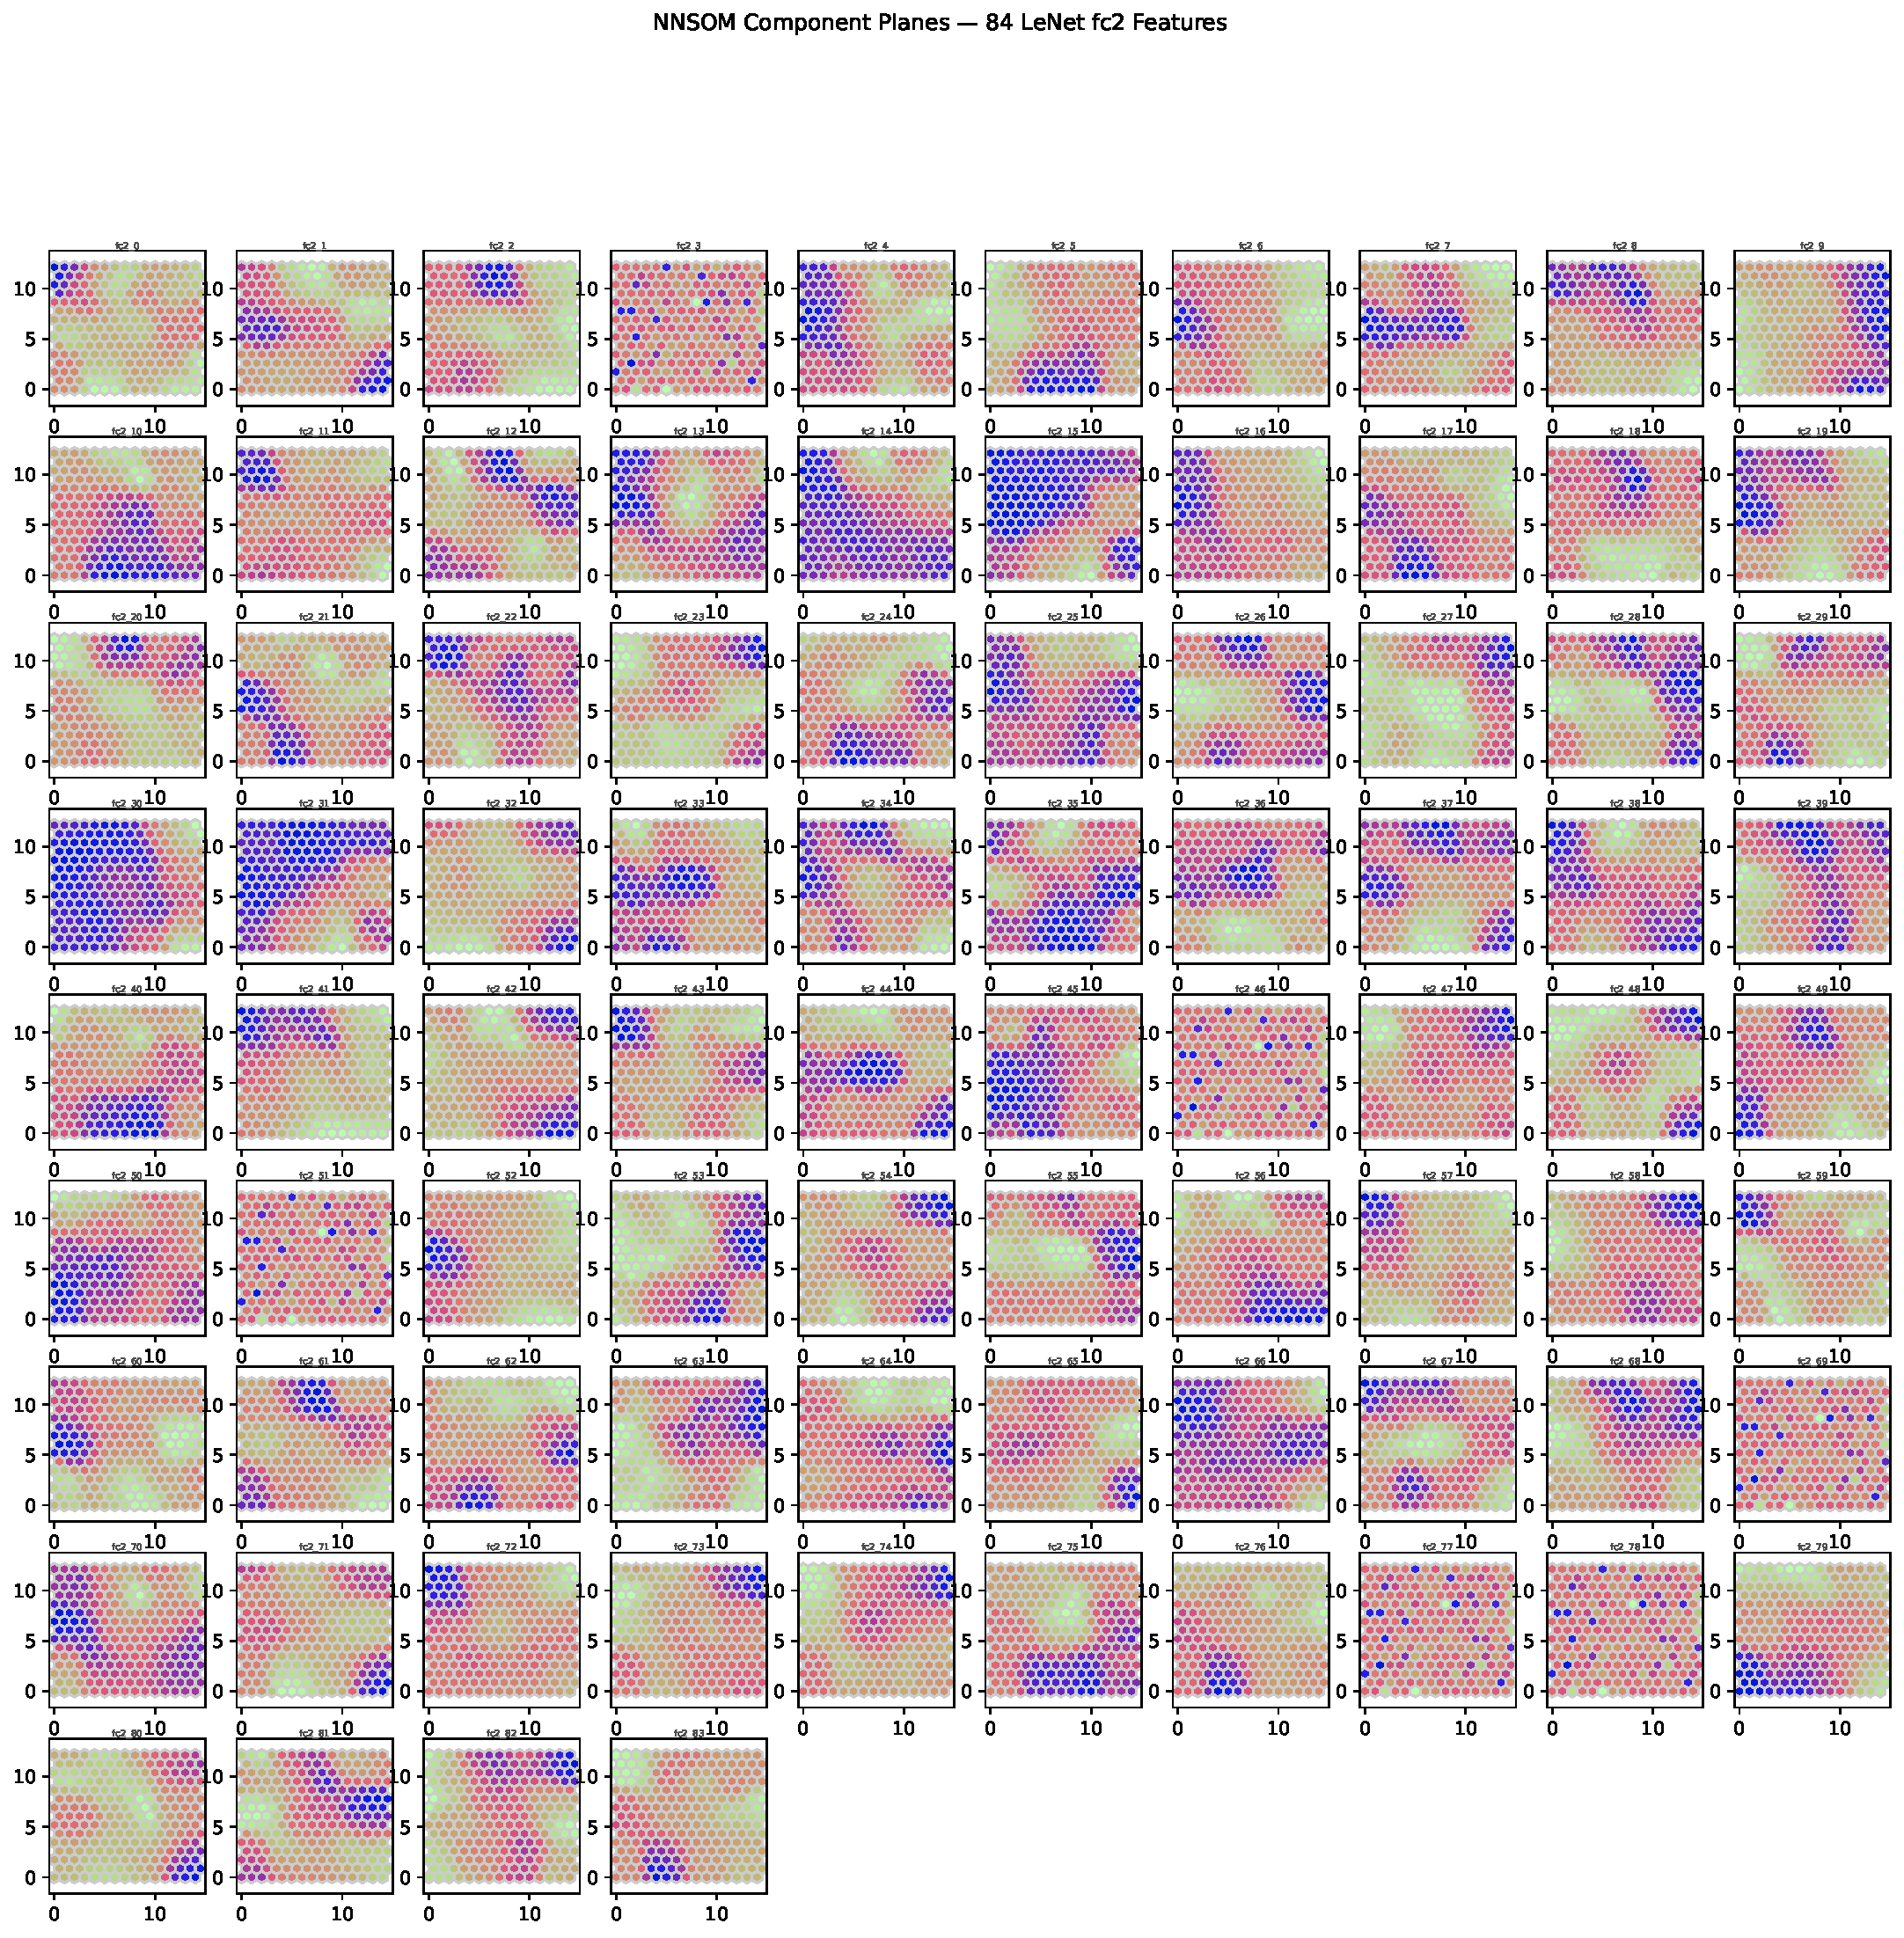
\includegraphics[width=0.94\textwidth]{component_planes_all84_nnsom.pdf}
    \caption{Overview of all 84 component planes for the trained SOM.}
\end{figure}

The experiment metadata identifies features 15, 19, 79, 41, 35, and 53 as
high-variance \texttt{fc2} dimensions. Two representative feature maps are used
in the main report to keep the presentation focused.

\begin{figure}[H]
    \centering
    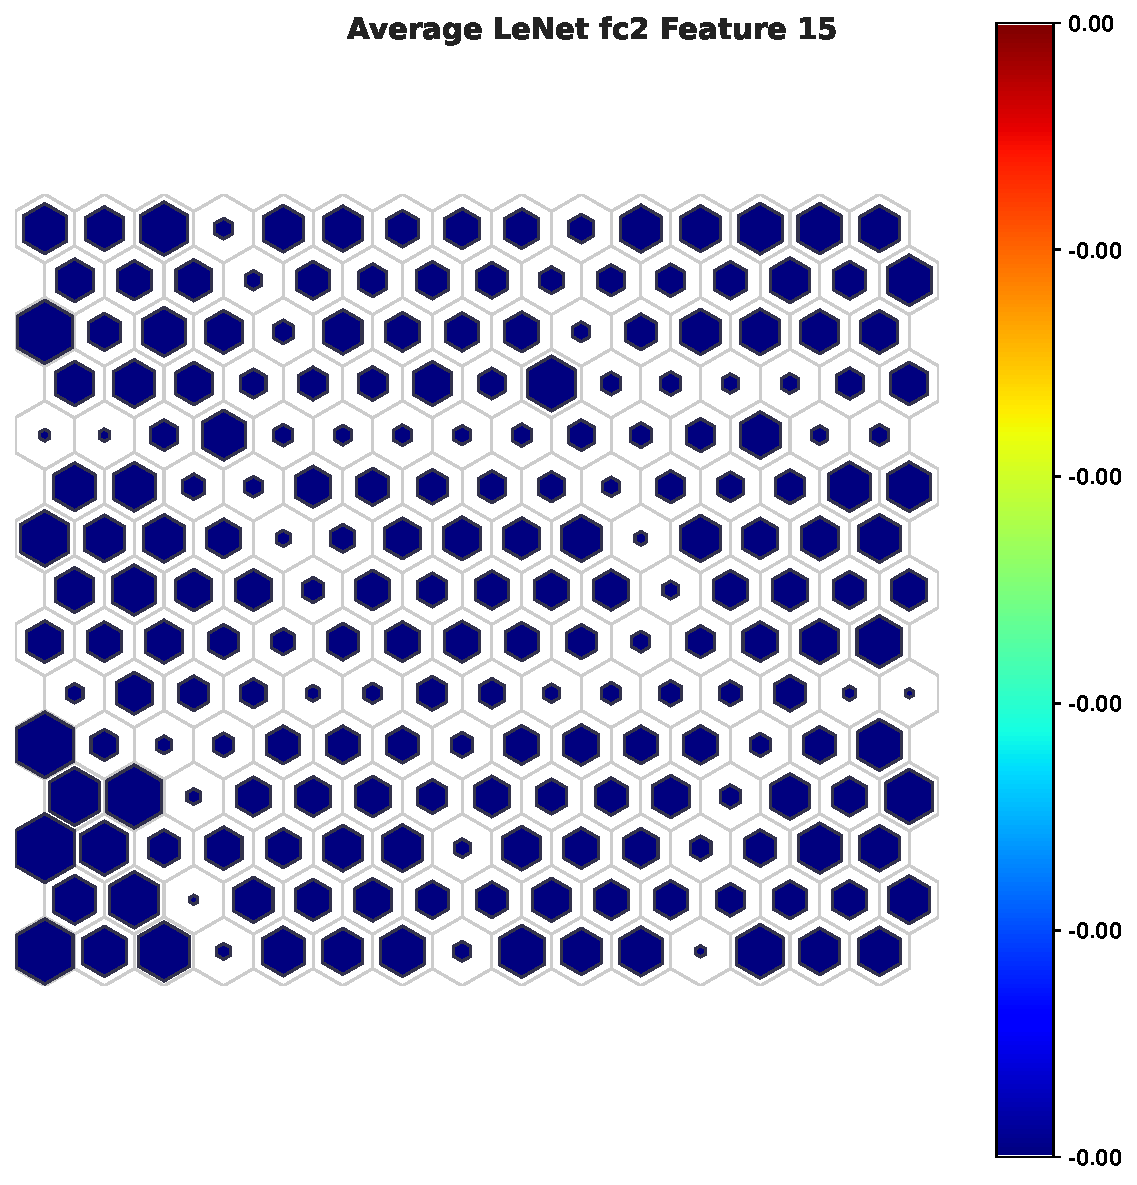
\includegraphics[width=0.47\textwidth]{fc2_15_color_hist.pdf}
    \hfill
    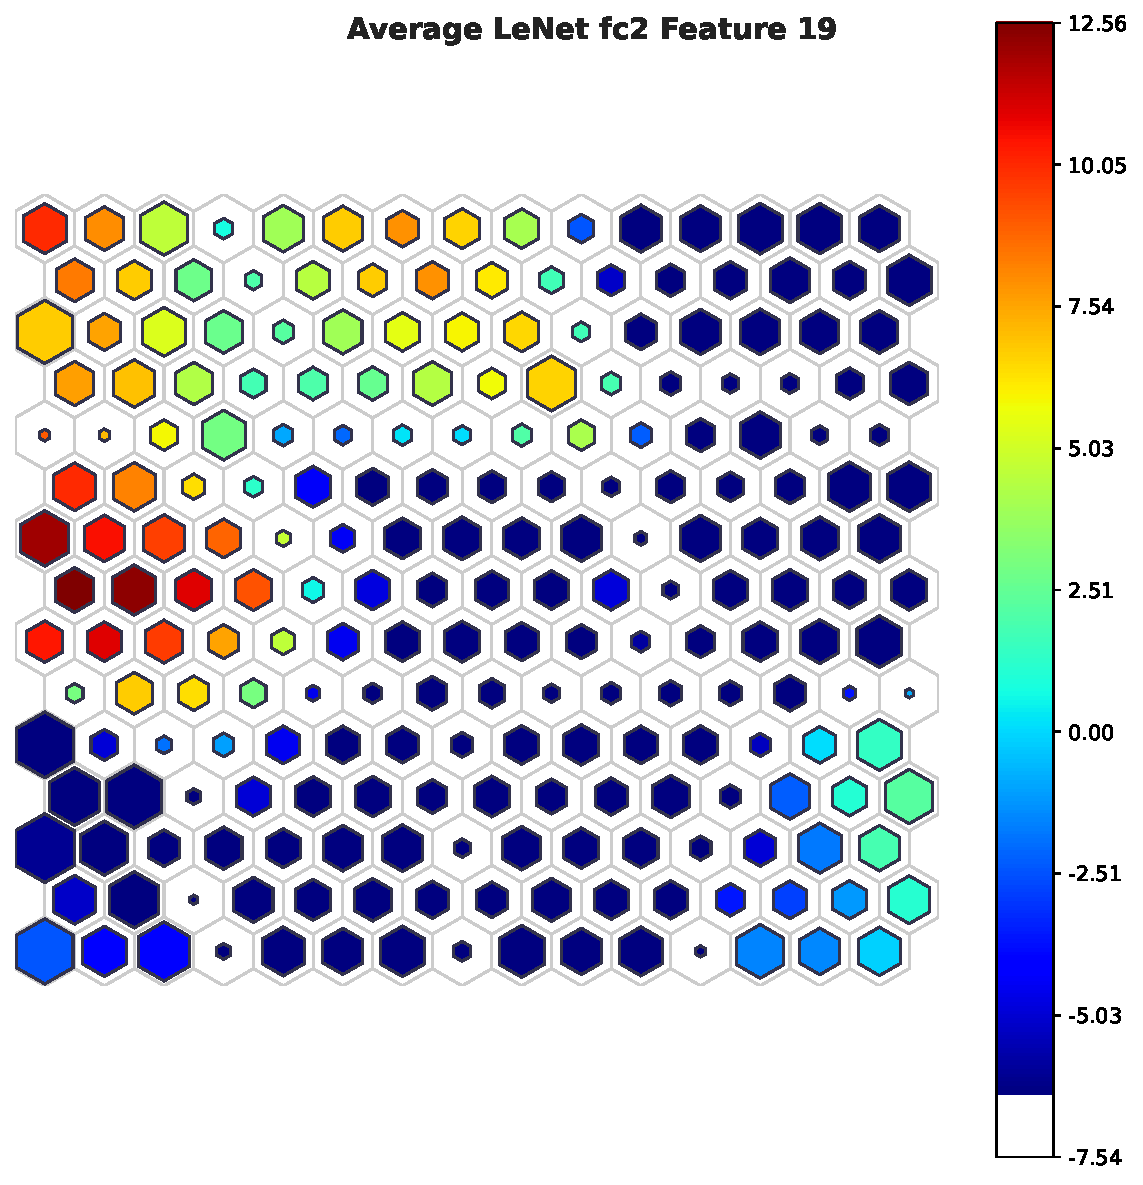
\includegraphics[width=0.47\textwidth]{fc2_19_color_hist.pdf}
    \caption{Representative high-variance \texttt{fc2} feature maps (features 15 and 19).}
\end{figure}

\section{Class Organization}

Class maps show where validation samples from individual digit classes land on
the SOM. They are useful for identifying compact regions, neighboring classes,
and areas of overlap. Two representative classes are shown here rather than
reproducing all ten maps.

\begin{figure}[H]
    \centering
    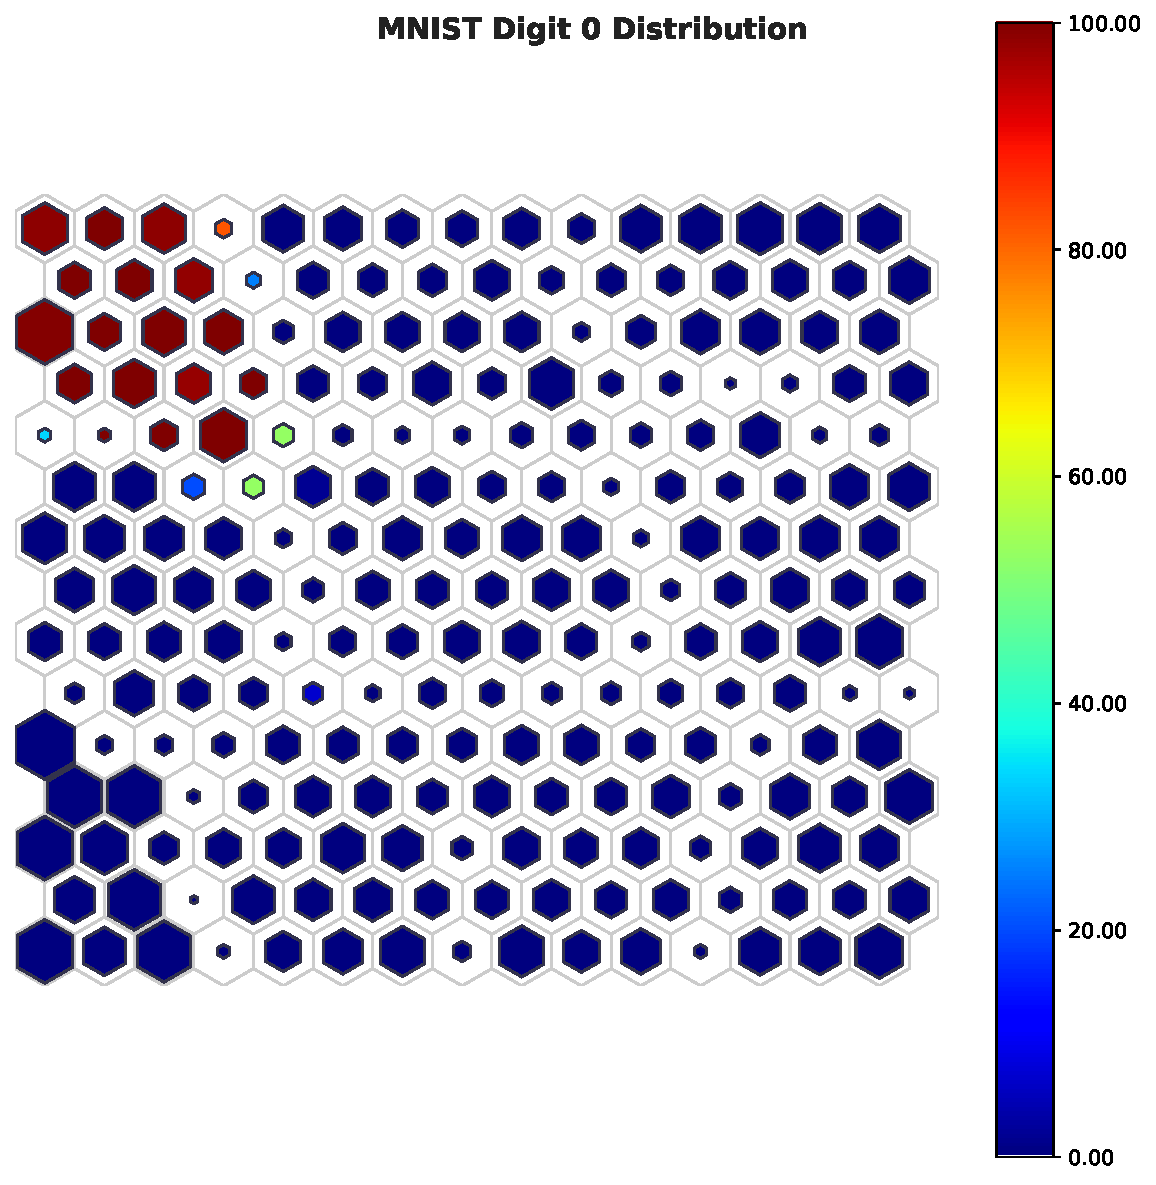
\includegraphics[width=0.47\textwidth]{digit_0_color_hist.pdf}
    \hfill
    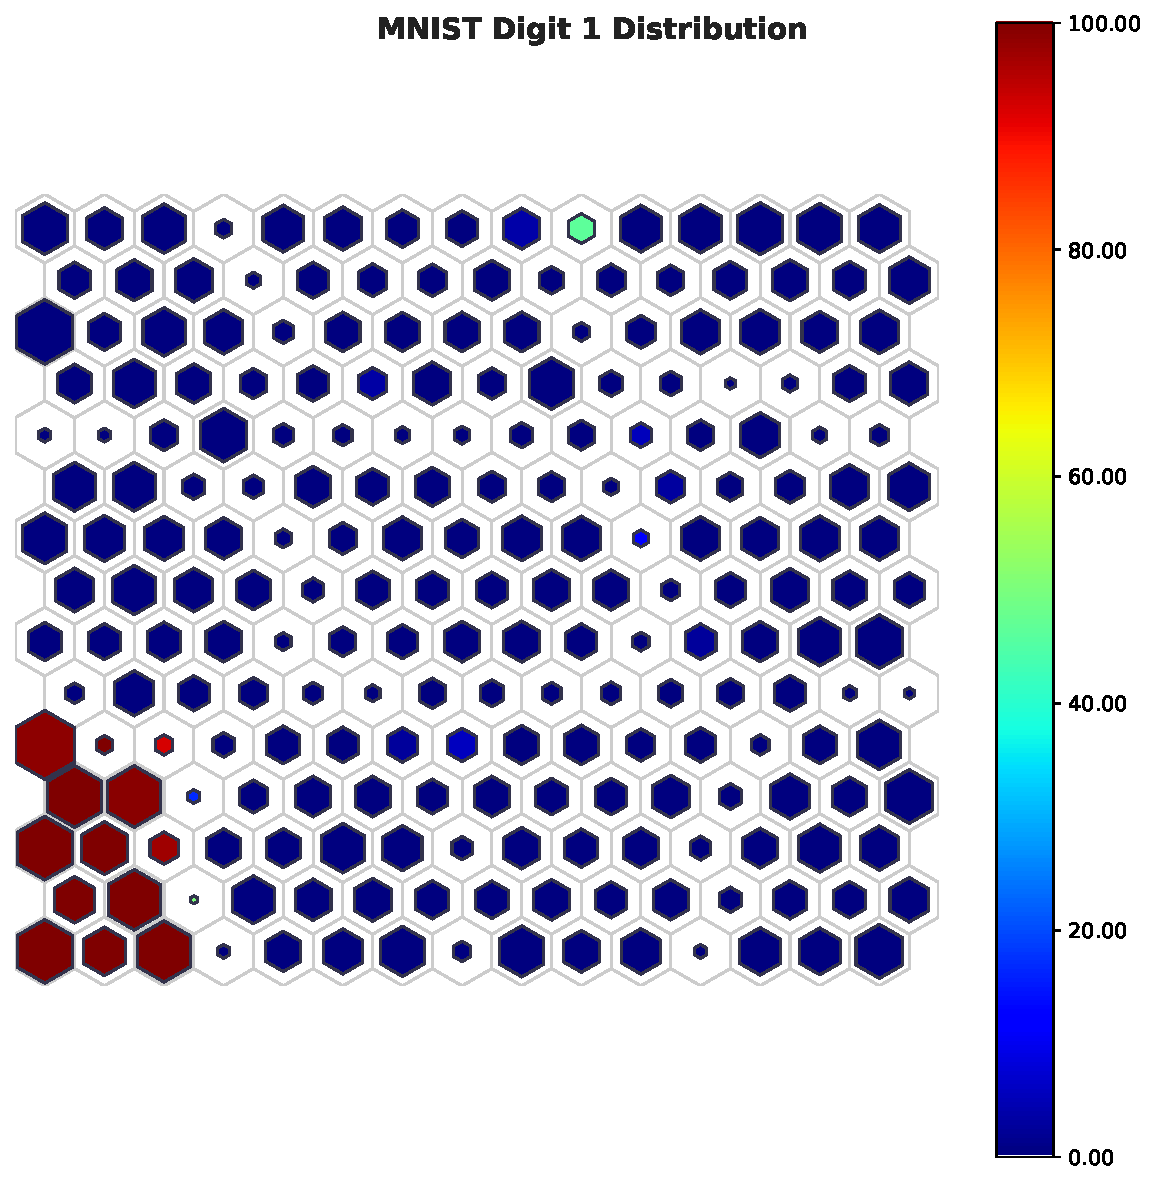
\includegraphics[width=0.47\textwidth]{digit_1_color_hist.pdf}
    \caption{Representative validation class maps for digits 0 and 1.}
\end{figure}

\section{Validation Error Geography}

The validation analysis maps connect SOM location with predictive quality.
The purity map summarizes class homogeneity within each neuron, while the
validation error-rate/support map localizes regions with weaker predictive
behavior. The combined error map provides a compact view of neurons that merit
targeted inspection.

\begin{figure}[H]
    \centering
    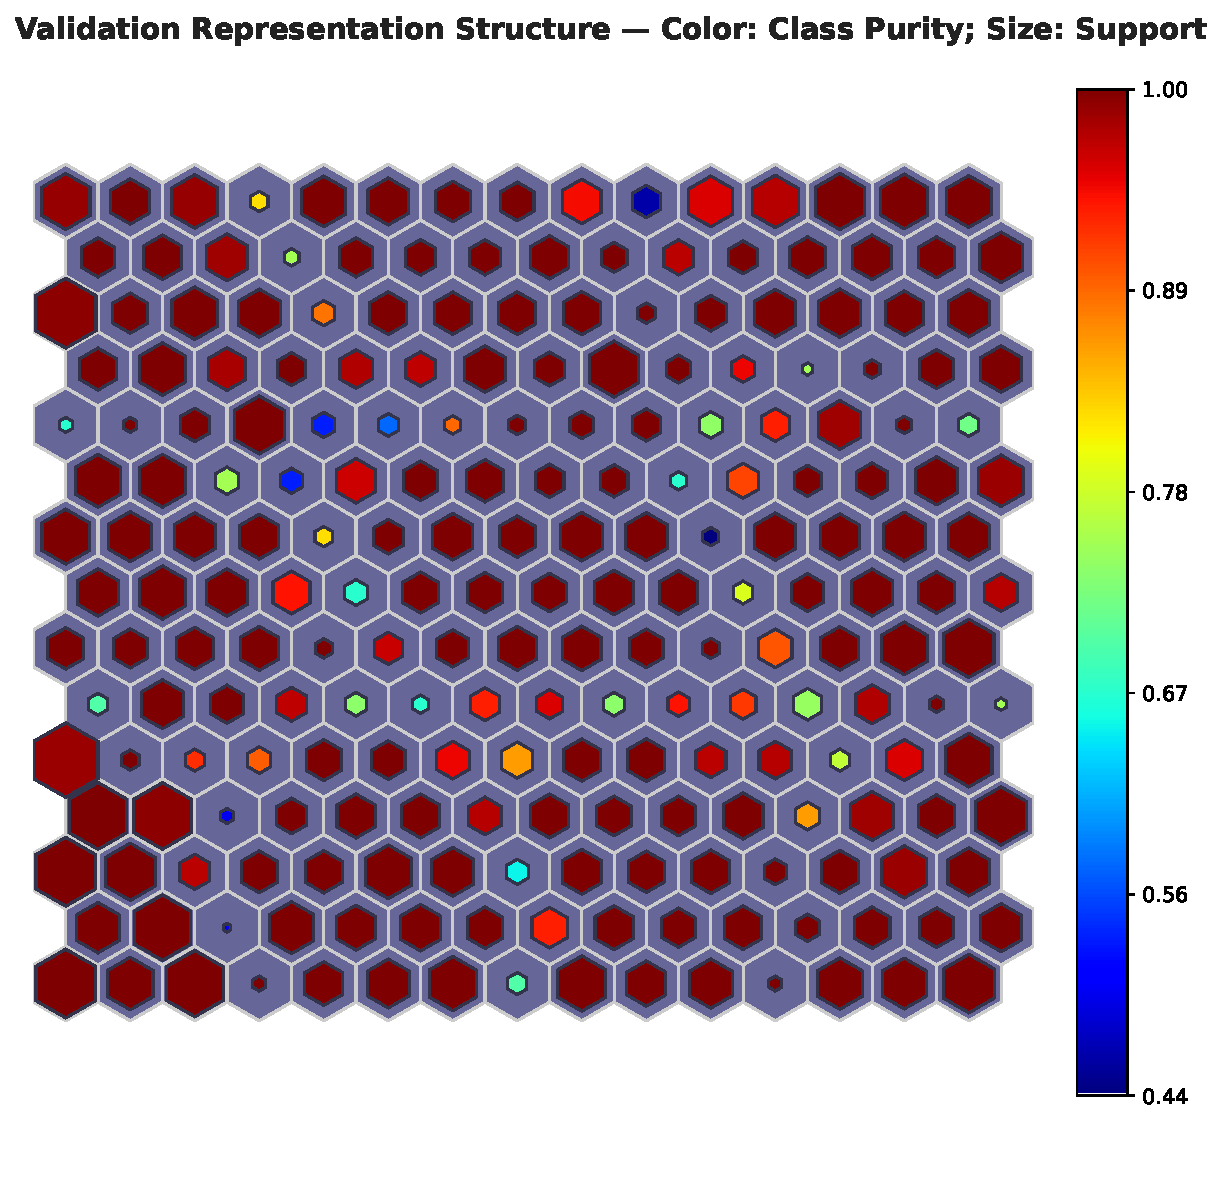
\includegraphics[width=0.47\textwidth]{validation_purity_support.pdf}
    \hfill
    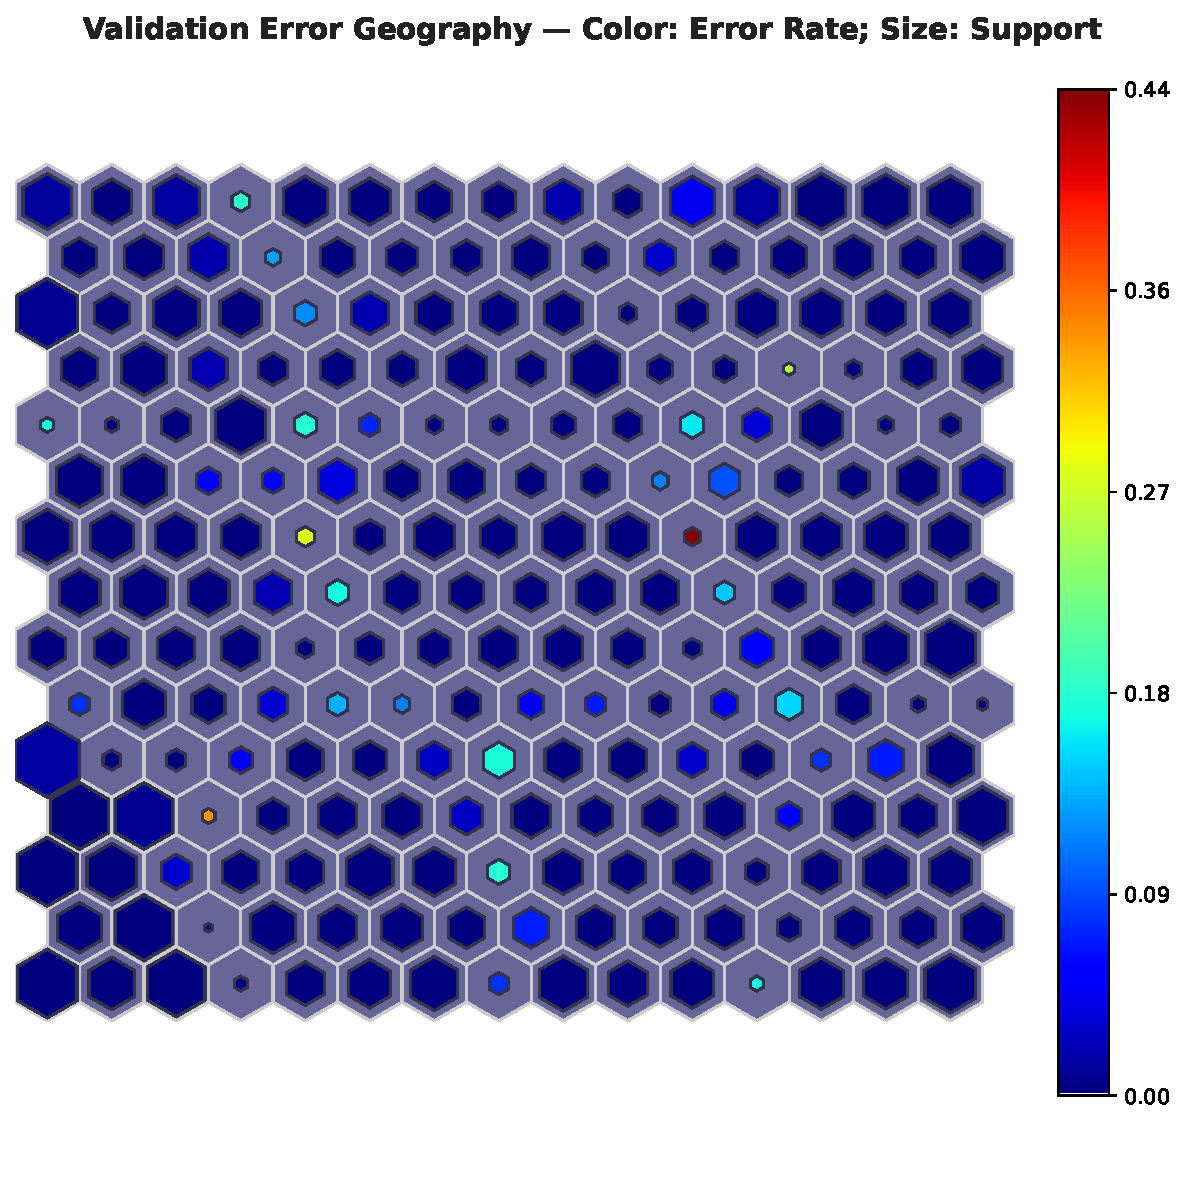
\includegraphics[width=0.47\textwidth]{validation_error_rate_support.pdf}
    \caption{Validation purity and validation error-rate/support maps.}
\end{figure}

\begin{figure}[H]
    \centering
    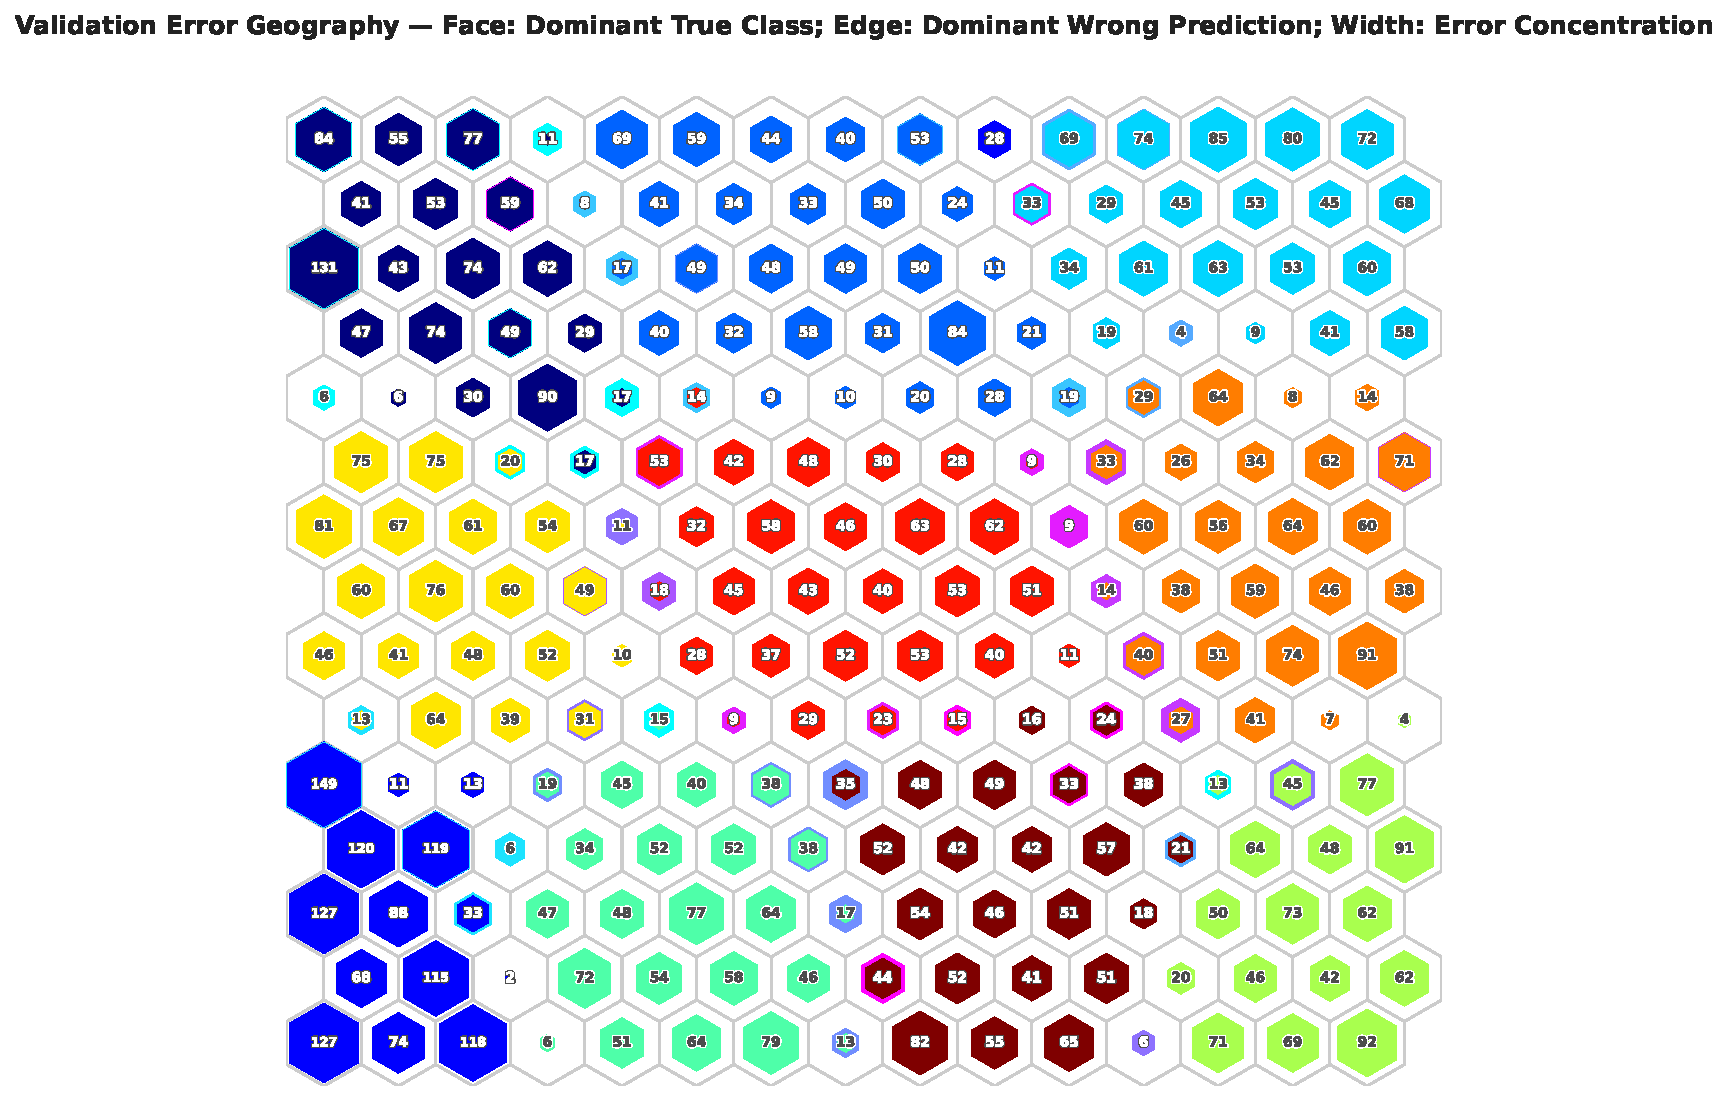
\includegraphics[width=0.78\textwidth]{validation_complex_error_map.pdf}
    \caption{Combined validation error-purity visualization for identifying candidate problem regions.}
\end{figure}

These visualizations identify candidate regions for later quantitative hotspot
analysis; they are not by themselves evidence that a neuron is an OOD detector
or that a SOM-guided intervention will improve predictive performance.

\section{Discussion}

The 15$\times$15 map provides a structured two-dimensional organization of the
CNN's 84-dimensional latent representation. The central question is whether
this organization contains information useful beyond visualization. The
U-Matrix, hit maps, component planes, class maps, and validation-quality maps
provide complementary views of topology, density, feature organization, class
organization, and local predictive behavior.

At this stage, the evidence is descriptive. Quantitative claims about error
hotspots, novelty detection, or retraining benefit require explicit neuron-level
statistics, calibrated thresholds, comparisons with established OOD/anomaly
baselines, and controlled before/after experiments. Visually coherent SOM
structure alone does not establish superior detection or predictive performance
\cite{hendrycks2017baseline,lee2018mahalanobis}.

\section{Conclusion and Next Phase}

The SOM 15$\times$15 experiment establishes the map structure needed for the
next stage of post-training analysis. The trained map organizes fixed CNN
embeddings into a topology that can now be evaluated quantitatively using BMU
occupancy, class purity, prediction error rates, quantization distances, and
neighborhood statistics.

The next phase should convert the visual observations into measurable
error-geography and novelty-detection experiments. Development decisions and
thresholds should be calibrated on training/validation data only, preserving
the final test set for unbiased evaluation.

\printbibliography[title={References}]

\end{document}
